%=================================================
% CHAPITRE 3 : Release 1
%=================================================

\chapter{Release 1 : Socle technique et moteur de données}

\section{Introduction}

La première release a été consacrée aux fondations de SIRH-Doc. Avant de travailler sur les documents eux-mêmes, il fallait résoudre deux problèmes plus profonds : sécuriser l'accès aux données et rendre ces données exploitables par une interface générique. Cette release regroupe donc le sprint 1, consacré au socle technique, et le sprint 2, consacré au moteur de données et aux entités métier.

\section{Sprint 1 : Socle technique, Multi-Tenancy et isolation temporelle}

\subsection{Objectif du sprint}

L'objectif du sprint 1 était de construire un socle fiable : authentification JWT, résolution du tenant, séparation des organisations et prise en compte de l'année universitaire. Ce travail était indispensable, car la plupart des fonctionnalités de SIRH-Doc dépendent du contexte de l'utilisateur connecté. Un document n'a pas la même signification selon l'établissement, l'année universitaire et les droits de l'utilisateur.

\subsection{Backlog du sprint}

% Tableau backlog sprint
\renewcommand{\arraystretch}{1.4}

\begin{longtable}{|>{\centering\arraybackslash}p{1cm}|
                  >{\raggedright\arraybackslash}p{10.4cm}|
                  >{\centering\arraybackslash}p{1.7cm}|}
\hline
\textbf{ID} & \textbf{User story} & \textbf{Priorité} \\
\hline

1 & En tant qu'utilisateur, je dois pouvoir me connecter et me déconnecter de la plateforme afin d'accéder à mon espace de travail. & Haute \\
\hline

2 & En tant qu'administrateur, je veux que les accès soient limités selon le rôle de chaque utilisateur afin de sécuriser les fonctionnalités de la plateforme. & Haute \\
\hline

3 & En tant qu'organisation, je veux que mes données soient isolées afin qu'aucun autre établissement ne puisse y accéder. & Haute \\
\hline

4 & En tant qu'utilisateur, je veux choisir l'année universitaire active afin de consulter et générer les documents dans le bon contexte. & Haute \\
\hline

5 & En tant que super administrateur, je dois pouvoir créer, modifier et consulter les organisations utilisant la plateforme. & Haute \\
\hline

\caption{Backlog du Sprint 1}
\label{tab:backlog_sprint1}

\end{longtable}

\subsection{Conception du sprint}

\begin{itemize}

    \item \textbf{Diagramme de cas d'utilisation}

    Le diagramme suivant illustre les principales interactions entre les utilisateurs et le système durant ce sprint. Il se concentre principalement sur l’authentification, la gestion des accès et la sélection du contexte de travail avant l’accès aux fonctionnalités métier.

    \begin{figure}[H]
        \centering
        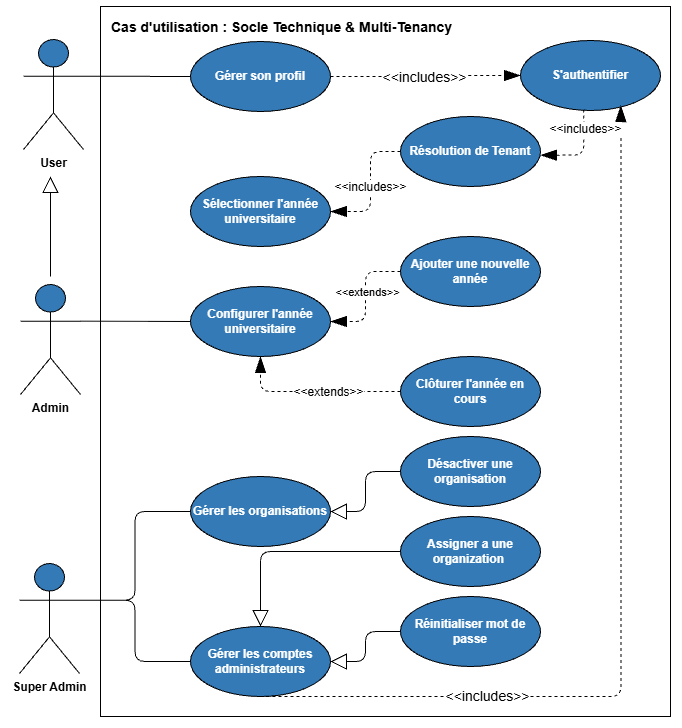
\includegraphics[width=0.9\textwidth]{images/sprint1/usecase-diagram.png}
        \caption{Diagramme de cas d'utilisation du Sprint 1}
        \label{fig:usecase-diagram-s1}
    \end{figure}

    % \item \textbf{Diagramme de classes}

    % Ce diagramme présente les principales entités persistantes du Sprint 1 ainsi que les relations qui structurent le socle technique de SIRH-Doc. Il met notamment en évidence la gestion des utilisateurs, des rôles, des organisations et du contexte académique nécessaires à l’isolation des accès et des données.

    % \begin{figure}[H]
    %     \centering
    %     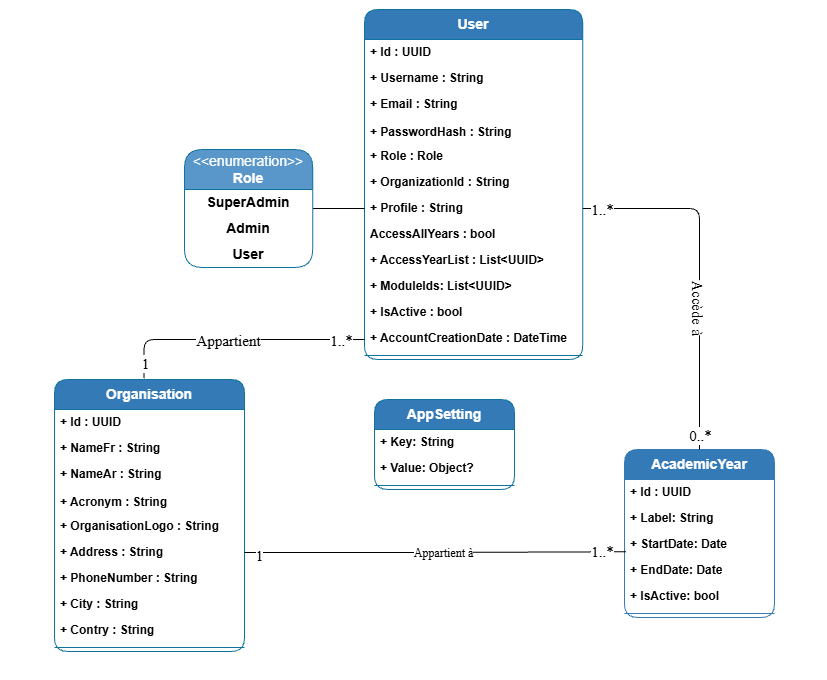
\includegraphics[width=0.95\textwidth]{images/sprint1/class-diagram.png}
    %     \caption{Diagramme de classes du Sprint 1}
    %     \label{fig:class-diagram-s1}
    % \end{figure}

    \item \textbf{Diagramme de séquence : Authentification JWT}

    Ce diagramme présente le processus d'authentification de l'utilisateur et la génération du jeton JWT permettant d'accéder à l'application.

    \begin{figure}[H]
        \centering
        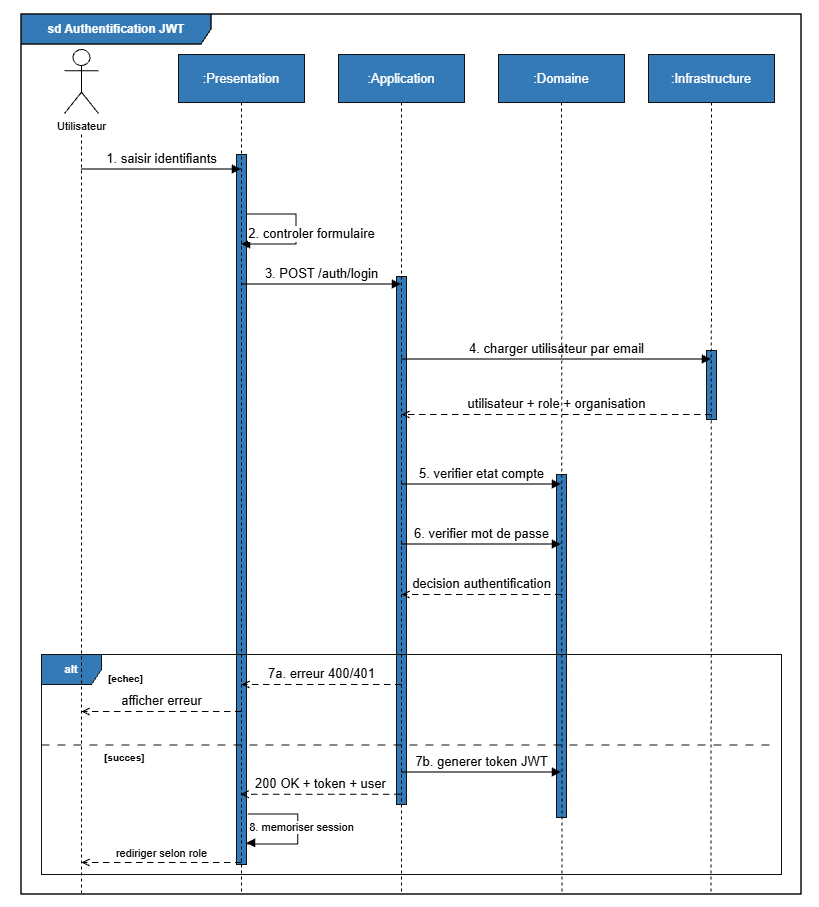
\includegraphics[width=0.95\textwidth]{images/sprint1/sequence-diagram1.png}
        \caption{Diagramme de séquence d’authentification JWT}
        \label{fig:jwt-sequence-s1}
    \end{figure}

    \item \textbf{Diagramme de séquence : Résolution dynamique du tenant}

    Ce diagramme illustre le mécanisme de résolution du tenant basé sur le jeton JWT lors de l'accès aux ressources protégées de la plateforme.

    \begin{figure}[H]
        \centering
        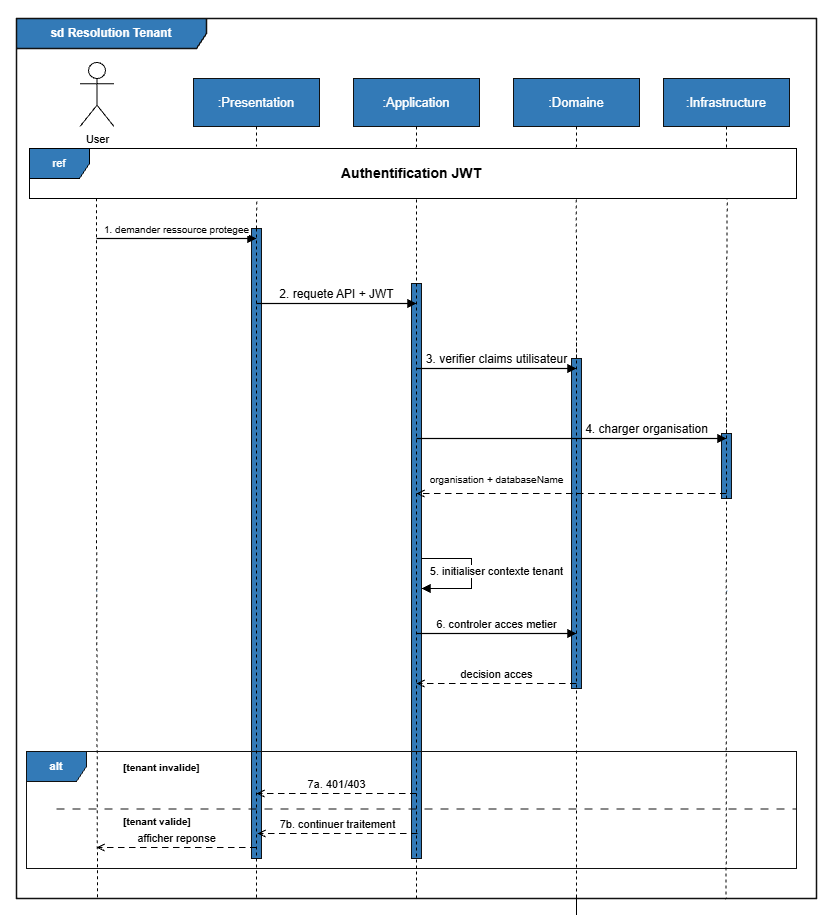
\includegraphics[width=0.95\textwidth]{images/sprint1/sequence-diagram2.png}
        \caption{Diagramme de séquence de résolution dynamique du tenant}
        \label{fig:tenant-sequence-s1}
    \end{figure}

\end{itemize}


\subsection{Réalisation du sprint}

La réalisation du Sprint 1 s'est concrétisée par les premières interfaces liées à l'accès sécurisé et au choix du contexte de travail. Ces écrans permettent de vérifier que l'utilisateur est bien authentifié, rattaché à une organisation et placé dans une année universitaire active avant d'accéder aux fonctionnalités métier.

\screenshotplaceholder{sprint1/login.png}{Page de connexion}{Interface de connexion à la plateforme}

La page de connexion constitue le premier point d'entrée de SIRH-Doc. Elle permet à l'utilisateur de saisir ses identifiants avant que le backend ne vérifie son compte, son rôle et son organisation.

\screenshotplaceholder[1\textwidth]
[1\textheight]{sprint1/academic-year-select.png}{Sélection de l'année universitaire}{Choix du contexte académique actif}

Après authentification, l'utilisateur sélectionne l'année universitaire active. Ce choix est important, car certaines données RH et pédagogiques doivent être consultées selon la période concernée.

\screenshotplaceholder[1\textwidth]
[1\textheight]{sprint1/home-by-role.png}{Ecran d'accueil}{Écran d’accueil principal}

Écran principal permettant à l’utilisateur d’accéder aux différents modules.

\screenshotplaceholder[1\textwidth]
[1\textheight]{sprint1/users-roles.png}{Gestion des utilisateurs et des rôles}{Interface de gestion des comptes utilisateurs}

La gestion des administrateurs et des organisations permet de définir des espaces dédiés à chacun. Elle vient compléter le dispositif d’authentification en rattachant chaque administrateur à un profil, à une organisation et à un périmètre d’intervention.

\section{Sprint 2 : Moteur de données et entités métiers}

\subsection{Objectif du sprint}

Le sprint 2 avait pour objectif de rendre l'application capable de gérer des données métier sans créer un écran spécifique pour chaque table. Dans un système RH universitaire, les entités peuvent être nombreuses : enseignants, vacataires, modules, grades, statuts, charges horaires, positions administratives. L'approche retenue est donc metadata-driven : la structure d'affichage et de filtrage est décrite par configuration.

\subsection{Backlog du sprint}

\renewcommand{\arraystretch}{1.4}

\begin{longtable}{|>{\centering\arraybackslash}p{1cm}|
                  >{\raggedright\arraybackslash}p{10.4cm}|
                  >{\centering\arraybackslash}p{1.7cm}|}
\hline
\textbf{ID} & \textbf{User story} & \textbf{Priorité} \\
\hline
\endfirsthead

\hline
\textbf{ID} & \textbf{User story} & \textbf{Priorité} \\
\hline
\endhead

6 & En tant que super administrateur, je dois pouvoir configurer les modules visibles dans l'application afin d'adapter la plateforme à chaque établissement. & Haute \\
\hline

7 & En tant que super administrateur, je dois pouvoir définir les colonnes, libellés, filtres et listes de valeurs d'une vue dynamique. & Haute \\
\hline

8 & En tant qu'utilisateur métier, je veux consulter les données des modules sous forme de tableaux paginés et filtrables. & Haute \\
\hline

20 & En tant qu'administrateur, je veux importer des fichiers de données avec validation afin de réduire la saisie manuelle et les erreurs. & Moyenne \\
\hline

\caption{Backlog du Sprint 2}
\label{tab:backlog_sprint2}

\end{longtable}

\subsection{Conception du sprint}

\begin{itemize}

    \item \textbf{Diagramme de cas d'utilisation}

    Le diagramme suivant illustre les interactions de l’administrateur avec les différents modules du système. Il décrit notamment les opérations de consultation, de filtrage, d’importation et de gestion des données métier.

    \begin{figure}[H]
        \centering
        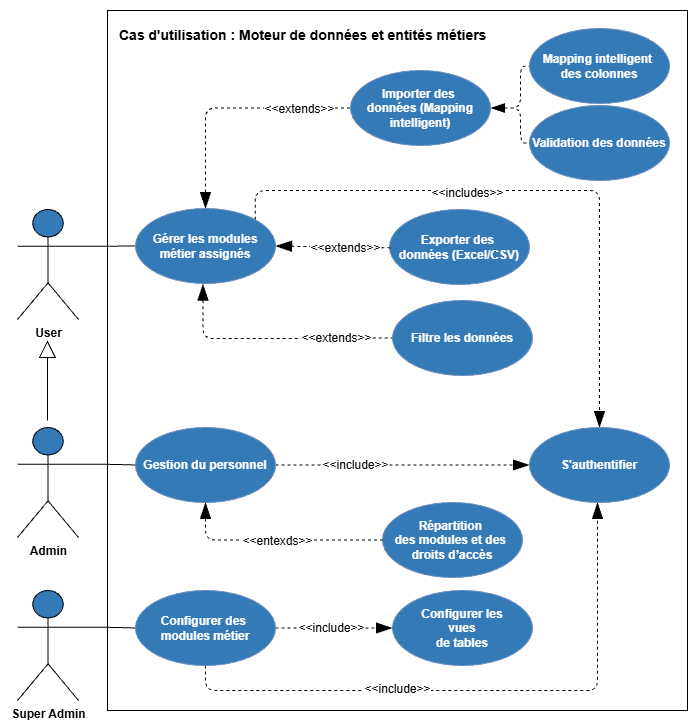
\includegraphics[width=0.9\textwidth]{images/sprint2/usecase-diagram.png}
        \caption{Diagramme de cas d'utilisation du Sprint 2}
        \label{fig:usecase-diagram-s2}
    \end{figure}

    % \item \textbf{Diagramme de classes}

    % Ce diagramme présente les principales entités introduites dans le Sprint 2 pour la gestion dynamique des données métier. Il met en évidence les configurations des modules, les vues dynamiques, les filtres ainsi que les structures utilisées pour l’importation et la consultation des données.

    % \begin{figure}[H]
    %     \centering
    %     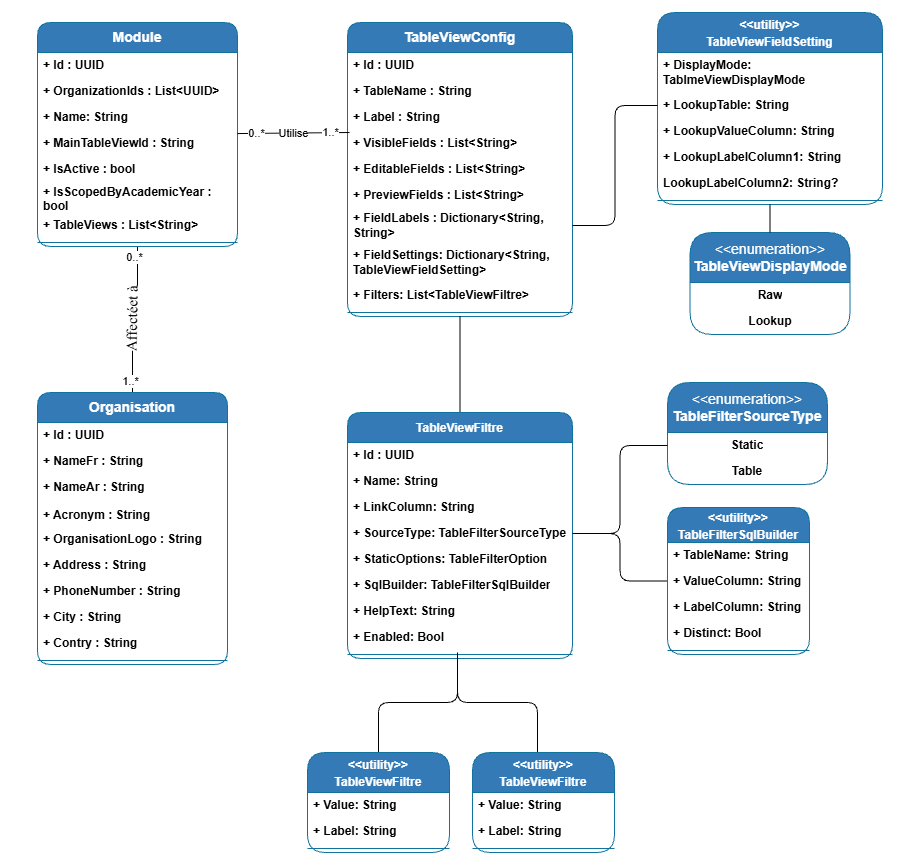
\includegraphics[width=0.95\textwidth]{images/sprint2/class-diagram.png}
    %     \caption{Diagramme de classes du Sprint 2}
    %     \label{fig:class-diagram-s2}
    % \end{figure}

    \item \textbf{Diagramme de séquence : Chargement d'une vue dynamique}

    Ce diagramme illustre le processus de chargement des données métier pour l'affichage dynamique des vues configurables.

    \begin{figure}[H]
        \centering
        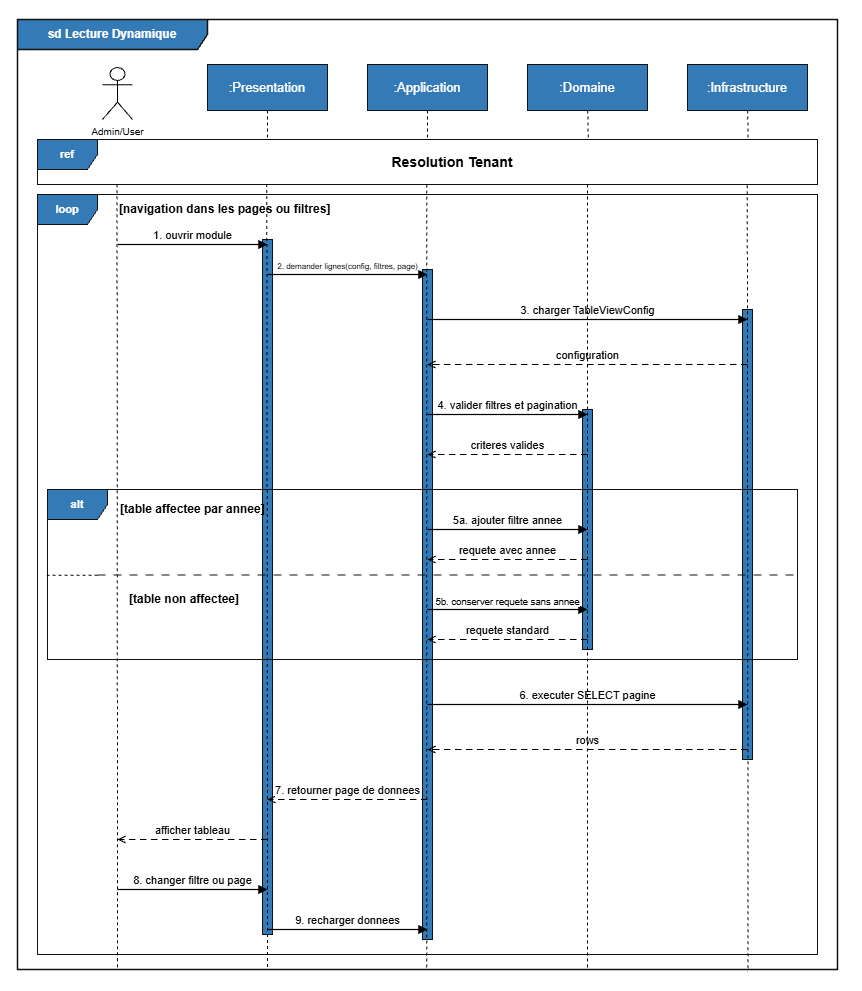
\includegraphics[width=0.95\textwidth]{images/sprint2/sequence-diagram1.png}
        \caption{Diagramme de séquence de chargement d'une vue dynamique}
        \label{fig:dynamic-view-sequence-s2}
    \end{figure}

    \item \textbf{Diagramme de séquence : Importation intelligente}

    Ce diagramme présente le fonctionnement de l'importation de fichiers de données avec contrôle de structure et validation métier.


    \begin{figure}[H]
        \centering
        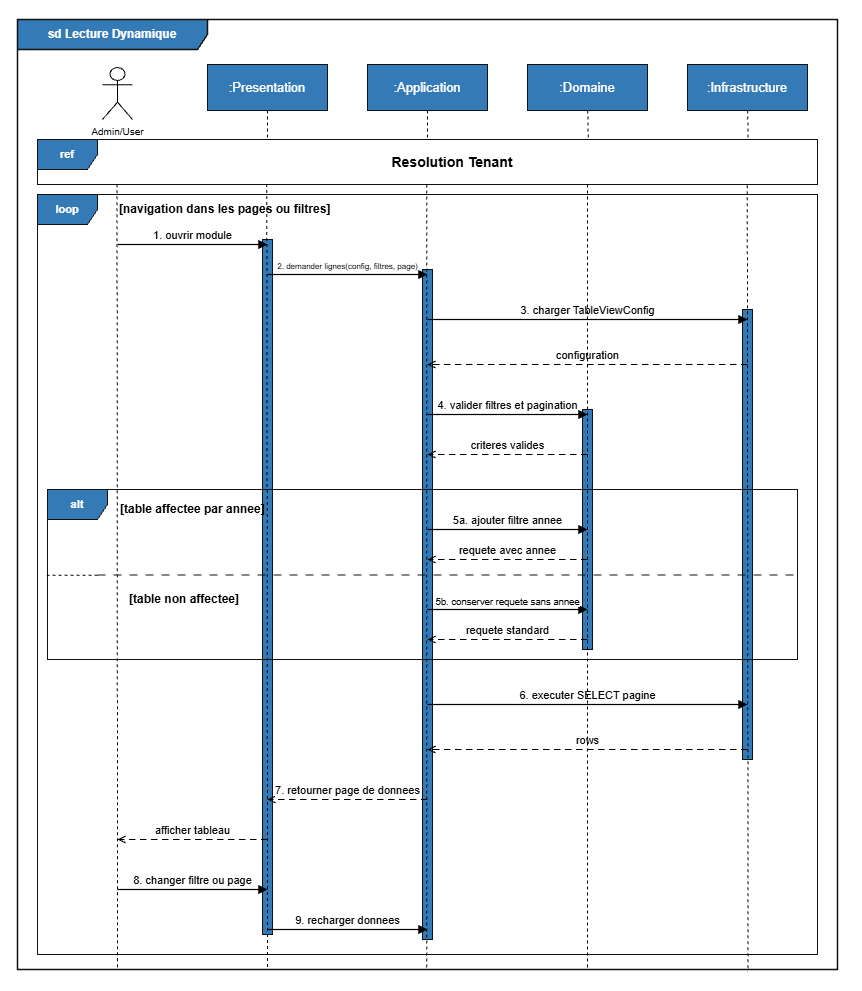
\includegraphics[width=0.95\textwidth]{images/sprint2/sequence-diagram2.png}
        \caption{Diagramme de séquence d’importation intelligente}
        \label{fig:import-sequence-s2}
    \end{figure}

\end{itemize}

\subsection{Réalisation du sprint}

Le Sprint 2 a été consacré aux interfaces de configuration et d’exploitation des données métier. L’objectif était de permettre au super administrateur de préparer les modules ainsi que les vues dynamiques, puis de laisser l’utilisateur consulter les données sous une forme claire, filtrable et paginée. Il s’agissait également de donner à l’administrateur la possibilité de restreindre l’accès à certaines données pour les utilisateurs non concernés.

\screenshotplaceholder[1\textwidth]
[1\textheight]{sprint2/config-module.png}{Gestion des modules}{Interface de configuration des modules}

\screenshotplaceholder[1\textwidth]
[1\textheight]{sprint2/config-tableview.png}{Configuration d'une TableView}{Paramétrage général d'une vue dynamique}

Ces interfaces donnent la possibilité au super administrateur de configurer l’approche metadata-driven.

\screenshotplaceholder[1\textwidth]
[1\textheight]{sprint2/module-vue.png}{Consultation dynamique d'un module}{Affichage paginé et filtrable des données métier}

La consultation et la manupulation dynamique montre le résultat de la configuration précédente côté utilisateur.

\screenshotplaceholder[1\textwidth]
[1\textheight]{sprint2/import.png}{Importation intelligente}{Sélection et préparation du fichier à importer}

L'importation intelligente enrichit le moteur de données en facilitant l’alimentation des tables métier.

\screenshotplaceholder[1\textwidth]
[1\textheight]{sprint2/personnel-management-module.png}{Gestion des accès aux modules}{Affectation des utilisateurs aux modules}

Le module de gestion du personnel illustre ensuite l'utilisation concrète d'un module métier par l'organisation. L'administrateur d'organisation peut enfin attribuer l'accès aux utilisateurs concernés, afin que chaque profil voie uniquement les modules liés à ses responsabilités et les données qu'il a l'acces.


\section{Conclusion Release 1}

À l'issue de la première release, SIRH-Doc dispose d'un socle sécurisé et d'un moteur de données configurable. Les décisions prises dans ces deux sprints conditionnent la suite du projet : le studio documentaire pourra s'appuyer sur des familles et des variables fiables, et la génération finale pourra exploiter des données déjà isolées par tenant et par année universitaire.
